\documentclass{article}\usepackage{noweb}\pagestyle{noweb}% ===> this file was generated automatically by noweave --- better not edit it
\usepackage{graphicx}
\begin{document}
\nwfilename{Board.nw}\nwbegindocs{1}\nwdocspar
\section{Introduction}
This file describes and implements various functionality related
to the board data structure used to represent the board in the
bagchal engine.

A board in the bagchal game is supposed to represent the state
of the game at an instant of time. The following are the components
that determine the state of the game:

\begin{itemize}

\item Whose turn is it?
\item The number of shikaar still left to be playes.
\item The number of shikaar that have already been killed.
\item The piece on each position on the board. i.e. Does the position
      (x, y) contain a tiger, or a shikaar, or is it empty?

\end{itemize}

While we could use a C-style structure to encode such a data
structure, experience with chess suggests that we use a bit-board
instead (see next paragraph). The bit-board is more flexible because
it acts as a hash function itself, in case we need indexing with the
board. Additionally manipulating the bit board is faster.

Here we are refering to the {\em bit-board} as a data-structure that
is a plain integer. The integer is intepreted according to the value of
the individual bit positions in its binary representation.

We will use a 64-bit integer (althogh we do not require all the bits) to
represent the board. The 64-bit integer is defined in \texttt{types.h}.
See types.nw.

\nwenddocs{}\nwbegincode{2}\moddef{*}\endmoddef\nwstartdeflinemarkup\nwenddeflinemarkup
  \LA{}board.h\RA{}

\nwendcode{}\nwbegincode{3}\moddef{board.h}\endmoddef\nwstartdeflinemarkup\nwenddeflinemarkup

#ifndef bagchal_engine_board_h
#define bagchal_engine_board_h

\LA{}includes\RA{}

\LA{}Board type definition\RA{}

\LA{}function prototypes\RA{}

#endif

\nwendcode{}\nwbegindocs{4}{\Tt{}types.h\nwendquote} is included for {\Tt{}i64{\_}t\nwendquote}, the 64 bit integer.

\nwenddocs{}\nwbegincode{5}\moddef{includes}\endmoddef\nwstartdeflinemarkup\nwenddeflinemarkup

#include <types.h>

\nwendcode{}\nwbegindocs{6}\nwdocspar
\section{The bit-board}

The bit-board has 4 parts.


The first part (bits 0 [lsb\footnote{least significant bit}] to bit 49)
is for the state of each position in the borad. These are divided into
pairs of bits. Each pair describes a single position. (00 = empty,
01 = tiger, 10 = shikaar, 11 = {\em undefined}) See figure~\ref{fig:bagchal-board}.
Position $(0, 0)$ is defined by bits 0 and 1. Position $(0, 1)$ is 
defiend by bits 2 and 3. Position $(x, y)$ is defined by bits

\[
b1 = 2x + 10y,\ b2 = 2x + y + 1,\ x, y \in \{0, 1, 2, 3, 4\}
\]

\begin{figure}

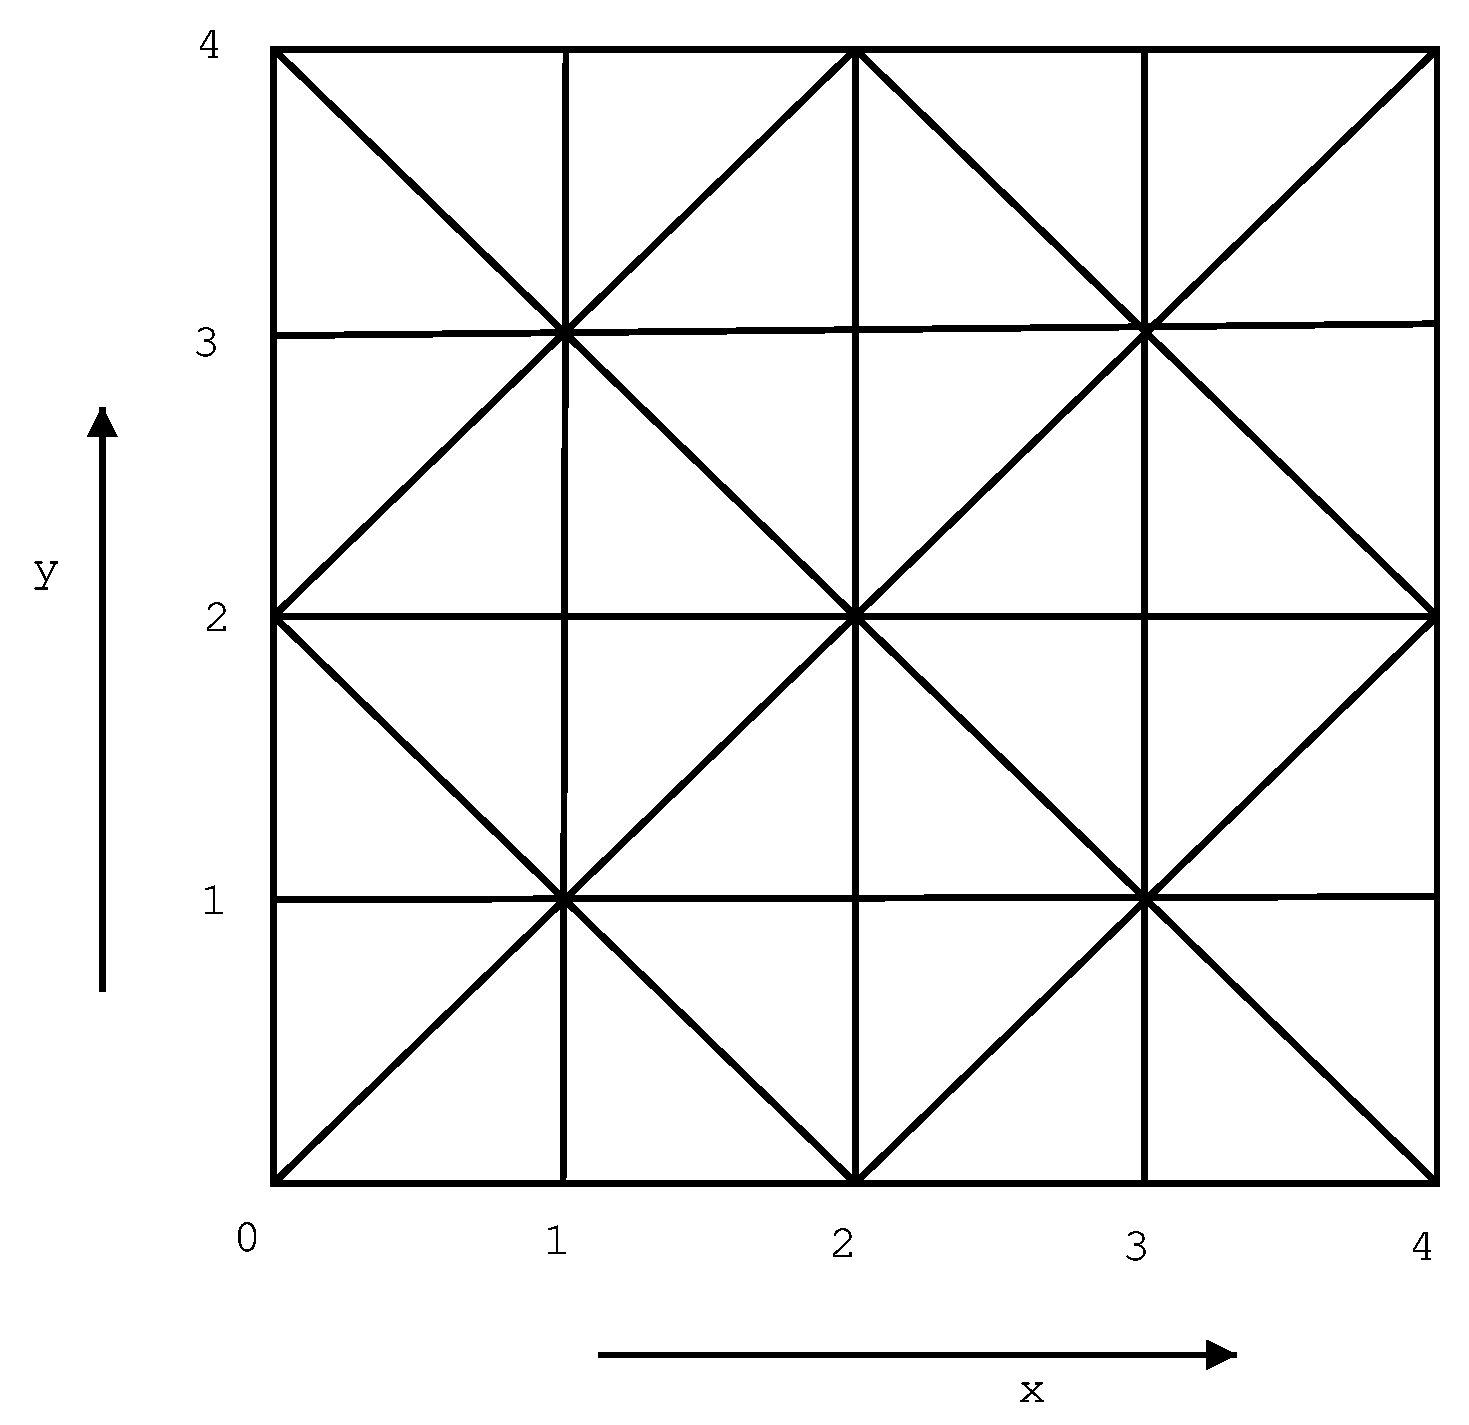
\includegraphics[scale=0.4]{Board.eps}
\caption{The empty bagchal board with co-ordinates}
\label{fig:bagchal-board}

\end{figure}



\end{document}
\nwenddocs{}
